\documentclass[12pt]{article}
\usepackage{geometry}
\usepackage{amsmath}
\usepackage{graphicx}

\title{COL780 : Computer Vision\\Background Subtraction}
\author{Suyash Agrawal\\2015CS10262}

\begin{document}
\maketitle
\section{Introduction}
In this assignment we had to implement Background Subtraction using mixture of Gaussian model.
This is the base model proposed by Strauffer and Grimson in their paper.\\
Background subtraction using gaussian mixture model is done by fitting k-gaussians on each pixel,
which model the pixel value distribution. These gaussians are fitted using E.M. algorithm and their
online approximation is used for performance.

\section{Implementation}
First attempt to implement background subtraction was done in python using loops. The algorithm implemented
was taken from \cite{hal} and the results were found to be poor. The main drawback was that the speed was very
slow and it took approx. 30 seconds to process just one 600x700 frame.\\
Further attempts were made to convert this program to use only matrix operations and no loops as matrix operations
are highly optimized in numpy library. The result was that the speed was now good but the code became quite complex.
This resulted in hard debugging sessions and less flexibility in experimentation.

Finally, the code was written in C++, so that loops could be used without performance degradation and this resulted
in easy experimentation and debugging sessions. I tested the algorithm for various values of hyper-parameters, whose
details are given in the next section.
\section{Observations and Results}
The testing of the program was done for various test videos like: remote controlled car video, people walking video,
webcam video, simple animated video. The results were also compared to the native implementation in OpenCV library.\\
The program basically had these hyperparameters:
\begin{itemize}
    \item K - The number of gaussians to model each pixel.
    \item $\alpha$ - The learning rate of the algorithm
    \item T - The term deciding the number of gaussians representing background
    \item std\_dev- The initial standard deviation of each gaussian.
    \item mean - The initial mean of each gaussian
\end{itemize}
The observations after experimentation were:
\begin{itemize}
    \item The initial std\_dev should be kept high. Small values of std\_dev resulted in false classification of background pixels
        as foreground pixels.
    \item The initial mean did not affect the performance much. In my implementation I set it to 0 initially. This might be because
        mean can be very easily modified by algorithm to any value and thus having little impact on performance.
    \item T is a very important factor. Setting its value to low (e.g. 0.1) resulted in almost all of the picture to be classified as
        foregroung, while setting to high values(e.g. 0.9) resulted in very little foreground points. The value that I got good 
        results with were around 06-0.8 .
    \item $\alpha$ (Learning Rate) is also important factor as it determined how much time steps the algorithm took to classify a pixel
        as background. Large value led to very sparse and disconnected foreground (as the pixels were quickly merged to background), while
        low values resulted in unnatural trails and disturbance in the output.
    \item K (number of gaussians) were a key factor for the performance of the algorithm. Low values of K (like 1-2) resulted in very poor
        performance as there were not enough gaussians to model complex environment like people walking in street, while setting large values
        (like 6-7) also result in degraded performance. The optimal values were around 3 and I got the best result by setting the parameter 3.
\end{itemize}

\begin{figure}
    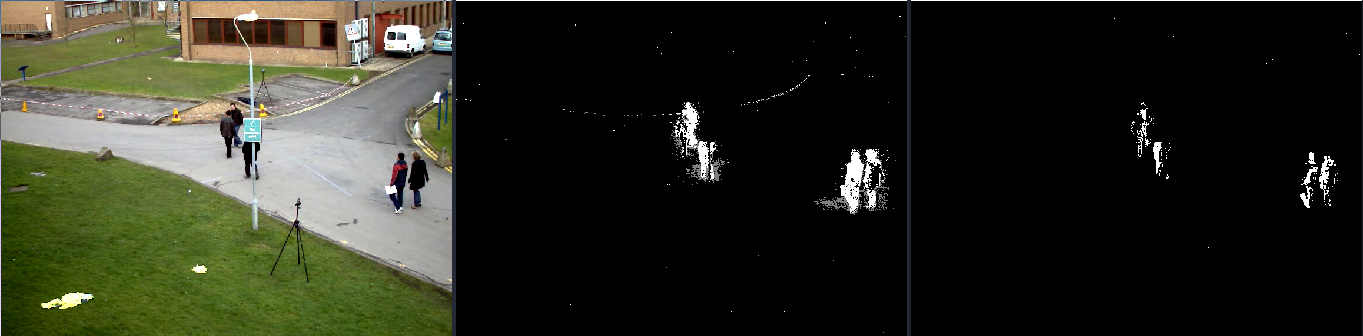
\includegraphics[width=\linewidth]{images/3/2017-09-18_03-43-01-1363x336.png}
    \caption{Result with 3 gaussians. (middle is opencv result)}
    \label{fig:boat1}
\end{figure}

\begin{figure}
    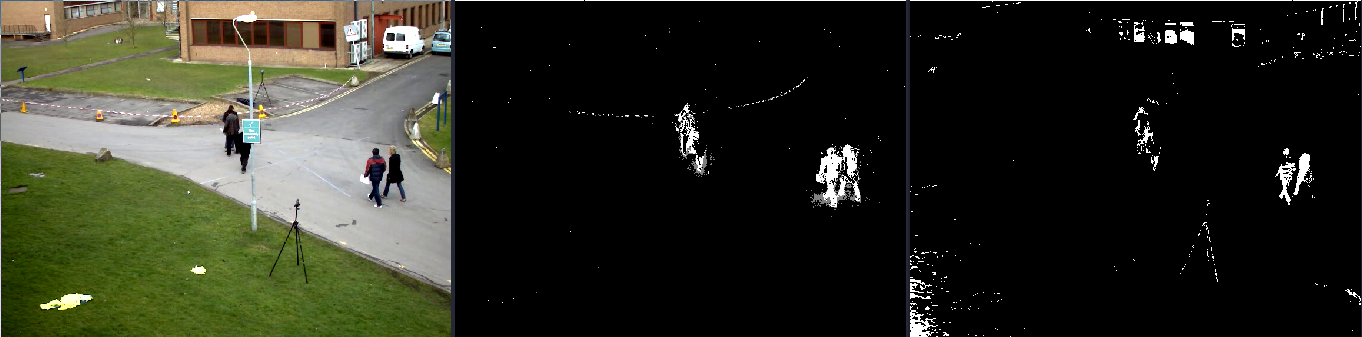
\includegraphics[width=\linewidth]{images/4/2017-09-18_03-36-54-1362x337.png}
    \caption{Result with 4 gaussians. (middle is opencv result)}
    \label{fig:boat1}
\end{figure}

\begin{figure}
    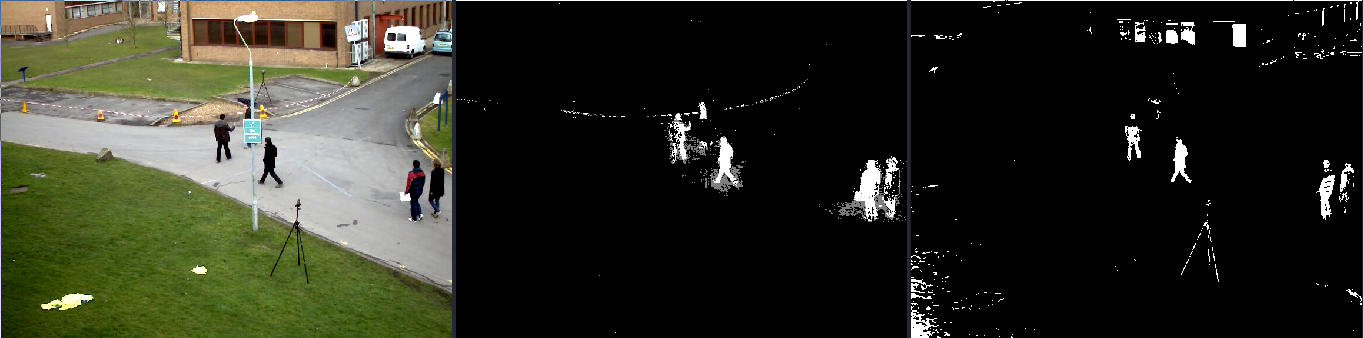
\includegraphics[width=\linewidth]{images/5/2017-09-18_03-33-02-1363x338.png}
    \caption{Result with 5 gaussians. (middle is opencv result)}
    \label{fig:boat1}
\end{figure}

\begin{figure}
    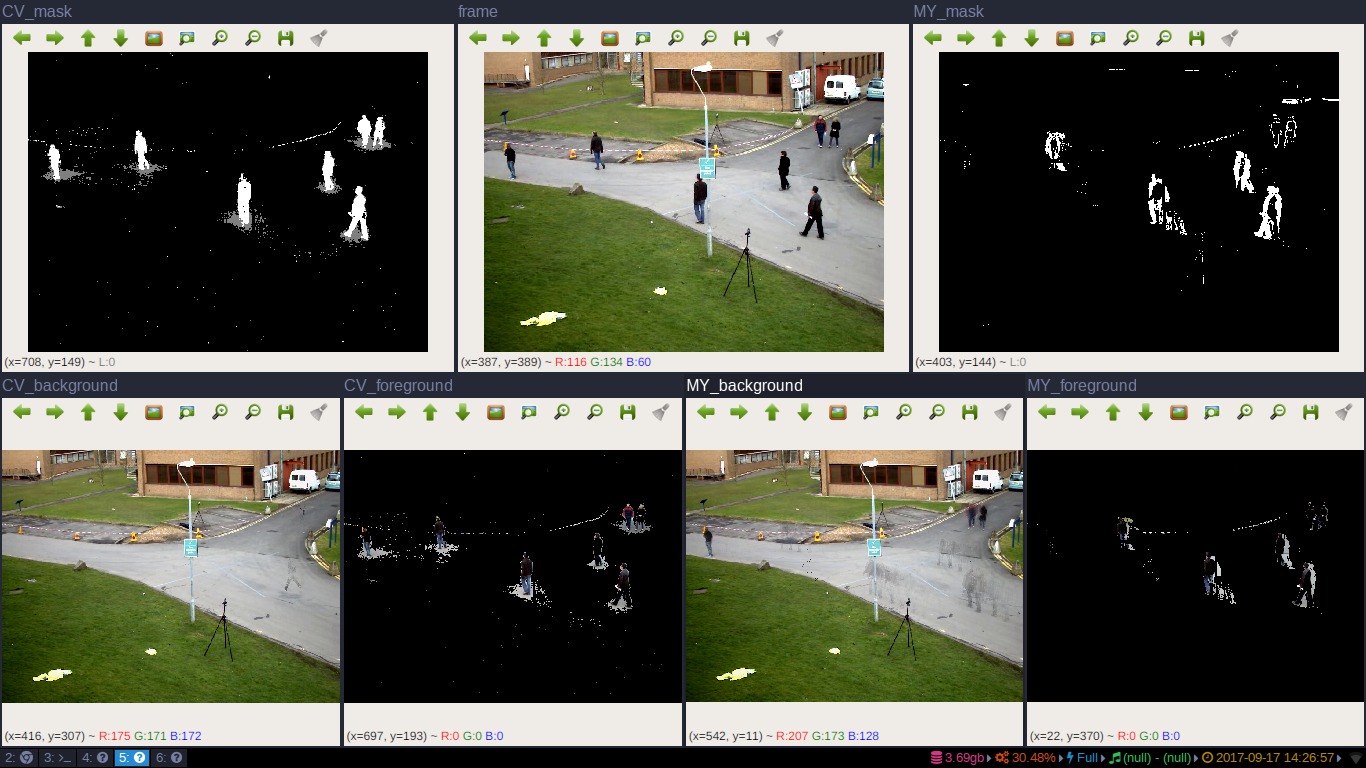
\includegraphics[width=\linewidth]{images/python/2017-09-17_14-26-58-1366x768.png}
    \caption{Result with pedestrian video in python implementation}
    \label{fig:boat1}
\end{figure}

\begin{figure}
    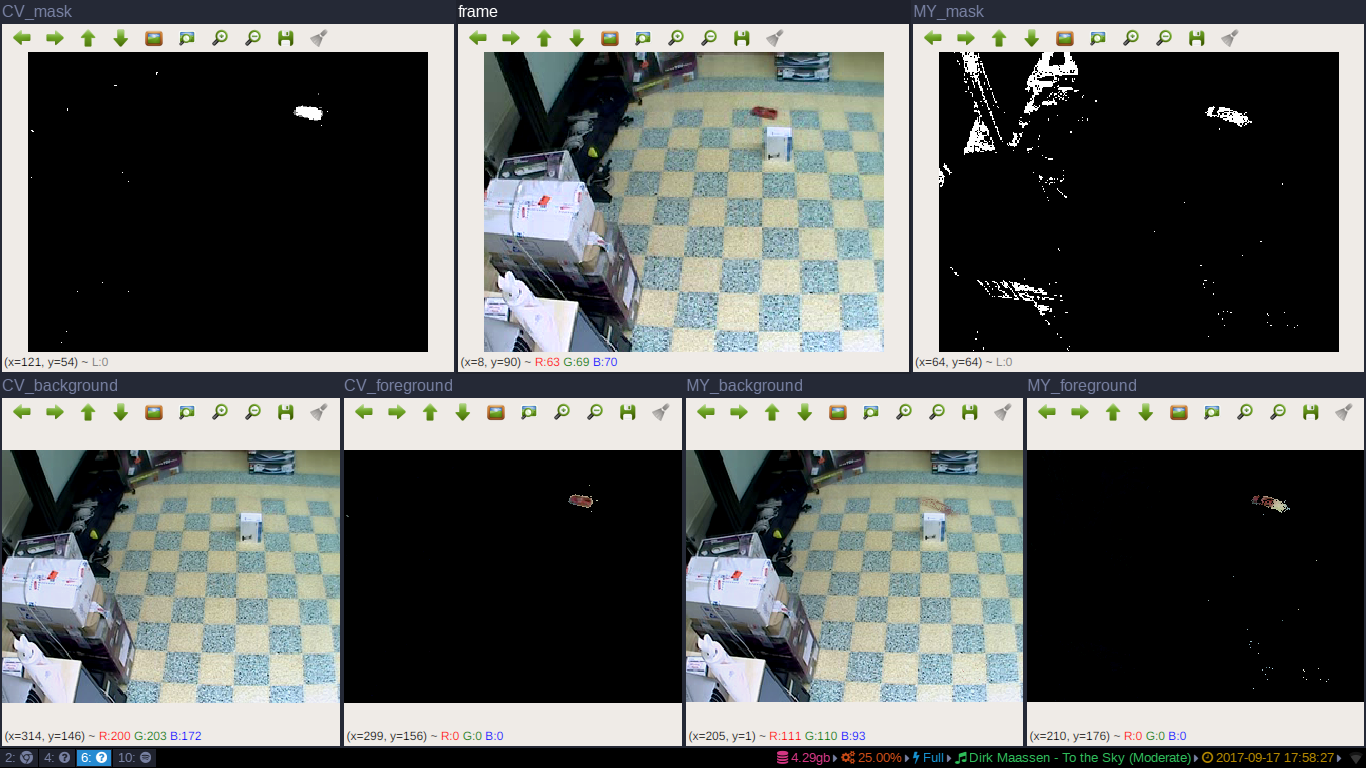
\includegraphics[width=\linewidth]{images/python/2017-09-17_17-58-28-1366x768.png}
    \caption{Result with car video in python implementation}
    \label{fig:boat1}
\end{figure}

\section{Conclusion}
I also found that OpenCV implementation was highly optimized, both in terms of speed and quality,
as compared to this algorithm. After a bit of research, I found that OpenCV's algorithm did not use a fixed number of gaussian for each
pixel and decided it dynamically along with various other optimizations. Also, it did all the operations in matrix form which gives a
huge speedup (as can be seen by me during python implementation).

In my experiments I found the results of OpenCV to be superior to mine. Though there were cases when OpenCV's output was fuzzier and
more delocalized than mine, but in general OpenCV results were very dense while my results, though very localized, were a bit sparse
and there were sometimes holes inside the objects.

\end{document}
